\section{Implementazione}

\subsection{Attributi dei File}
\begin{sitemize}
    \item \textbf{Nome:} Identificativo del file per l'utente.
    \item \textbf{Identificativo:} Etichetta unica utilizzata dal file system.
    \item \textbf{Tipo:} Specifica il tipo dei dati contenuti nel file, ad esempio testi, immagini, video oppure programmi.
    \item \textbf{Locazione:} Puntatore alla posizione del file sul dispositivo di memoria secondaria.
    \item \textbf{Dimensione:} Attuale dimensione del file.
    \item \textbf{Protezione:} Parametri di controllo su lettura/scrittura/esecuzione del file.
    \item \textbf{Ora, data, identificazione dell'utente:} Informazioni utili alla protezione del file.
\end{sitemize}

\begin{note}
    Gli attributi estesi sono una serie di informazioni aggiuntive che possono essere associate ad un file, essi sono una serie di coppie nome-valore e possono essere definiti dall'utente.

    Non vegnono salvati nel file, ma vengono salvati separatamente e gestiti dal file system.
\end{note}

\subsection{Tipo del File}
Il tipo del file è un attributo che indica la struttura interna e permette al sistema operativo di gestire il file in modo corretto.

\spacer
Le estensioni possono essere specificate in vari modi:
\begin{sitemize}
    \item Meccanismo delle estensioni (Windows)
    \item Attributo nella directory (MacOS)
    \item Valore posto all'inizio del file (Unix)
\end{sitemize}

\begin{figure}[H]
    \centering
    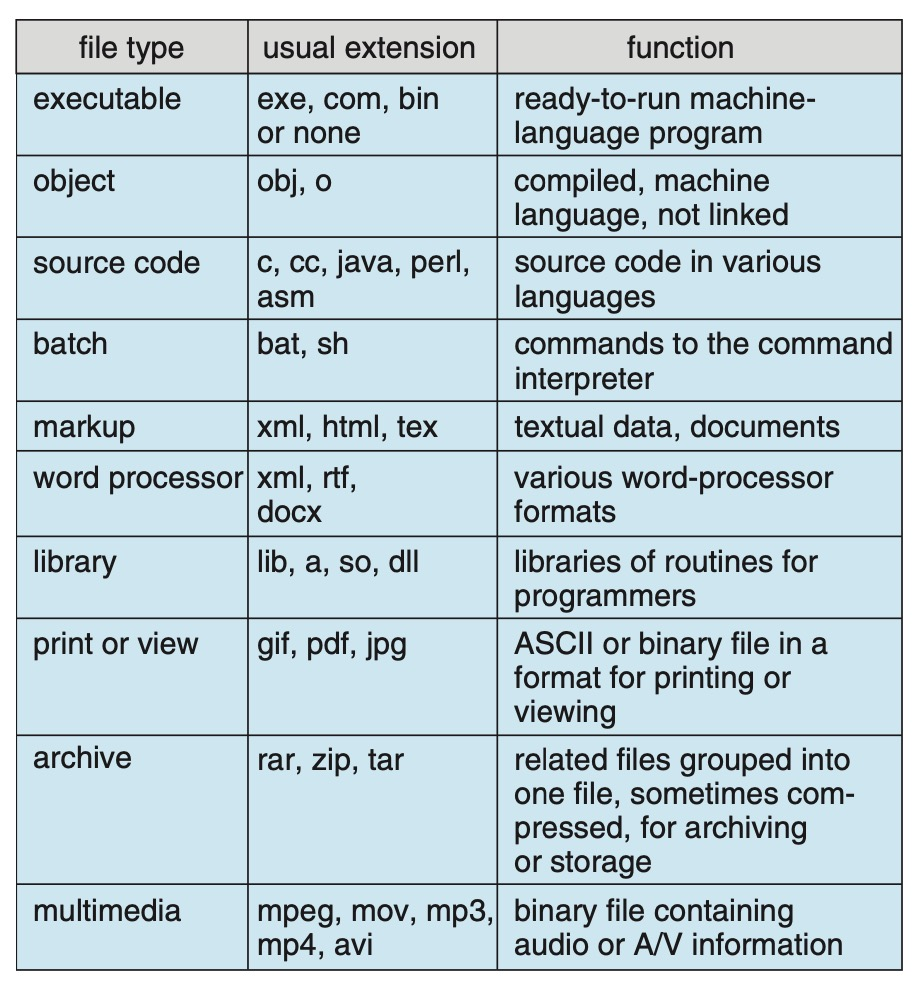
\includegraphics[width=0.5\linewidth]{assets/tipi-file.jpg}
\end{figure}

\subsection{Struttura del File}
Strettamente collegato al tipo del file, il quale può suggerirci la sua struttura interna.
\begin{sitemize}
    \item Nessuna Struttura (sequenza di byte)
    \item Struttura a record semplice (Linee a lunghezza fissa/variabile simili alle tabelle sql)
    \item Struttura complessa (documento formattato o eseguibile rilocabile)
\end{sitemize}

\spacer
Spesso è inefficiente lasciare al sistema operativo il compito di gestire ogni tipo di file, è più conveniente che esso sappia gestire solo i tipi base (spesso solamente i file eseguibili) e il resto viene lasciato a programmi di sistema o di terze parti.

Unix e DOS implementano questa scelta, i file sono gestiti solamente come stringhe di byte.

